\begin{question}{Problem 7.19 $\bigstar$}
Show that $\mathit{PRIMES}=\{m\mid m\text{ is a prime number in binary}\}\in\NP$. (Hint: For $p>1$, the multiplicative group $\mathbb{Z}_p^*=\{x\mid x\text{ is relatively prime to $p$ and }1\le x<p\}$ is both cyclic and of order $p-1$ iff $p$ is prime. You may use this fact without justifying it. The stronger statement $\mathit{PRIMES}\in\cP$ is now known to be true, but it is more difficult to prove.)
\end{question}
\begin{soln}
\textbf{Idea.} Trial division up to $\sqrt{m}$ is exponential in the \emph{binary} length $|m|=\Theta(\log m)$. A short \emph{Pratt certificate} exhibits a generator of $\mathbb{Z}_m^*$ together with a prime factorization of $m-1$, recursively certified; the hint then forces $m$ prime. Modular exponentiation (Problem~7.13) verifies the arithmetic in polynomial time.

\paragraph{Certificate.}
For $p=2$ the certificate is empty. For an odd integer $p>2$, a certificate $C(p)$ is a tuple
\[
\bigl(g;\; q_1,a_1,C(q_1);\; \dots;\; q_k,a_k,C(q_k)\bigr)
\]
where $g\in\{1,\dots,p-1\}$, the $q_i$ are distinct integers, $a_i\ge 1$, $p-1=\prod_i q_i^{a_i}$, and each $C(q_i)$ is a certificate that $q_i$ is prime.

\paragraph{Verifier $V$.}
$V=$ ``On input $\enc{p,C}$:
\begin{enumerate}
\item If $p=2$, \emph{accept}. If $p\le 1$, \emph{reject}.
\item Parse $C$ as $(g;q_1,a_1,C_1;\dots;q_k,a_k,C_k)$. Check $p-1=\prod_i q_i^{a_i}$ and $1\le g<p$ and $\gcd(g,p)=1$ (Euclid, Theorem~7.15).
\item Using repeated squaring $\bmod p$ (Problem~7.13), check $g^{p-1}\equiv 1\pmod{p}$ and $g^{(p-1)/q_i}\not\equiv 1\pmod{p}$ for every $i$.
\item Recursively run $V$ on each $\enc{q_i,C_i}$. Accept iff every recursive call accepts.''
\end{enumerate}

\paragraph{Why this certifies primality.}
If all checks pass, then $g\in\mathbb{Z}_p^*$ and the order of $g$ is exactly $p-1$ (it divides $p-1$ and is not a proper divisor, by checking prime factors). So $p-1$ divides $|\mathbb{Z}_p^*|=\varphi(p)\le p-1$, hence $\varphi(p)=p-1$ and $\mathbb{Z}_p^*$ is cyclic of order $p-1$. By the hint, $p$ is prime.

Conversely, if $p$ is prime then $\mathbb{Z}_p^*$ is cyclic of order $p-1$, so a generator $g$ exists, $p-1$ has a prime factorization, and we may attach recursive certificates for the $q_i$. Thus every prime has a certificate.

\paragraph{Size and time are polynomial in $|p|=\Theta(\log p)$.}
Along any branch of the factorization tree the integers strictly decrease, and in the worst case $p-1=2q$ with $q$ prime, so $q\le p/2$. The depth is therefore $O(\log p)$. At each node the written integers total $O(\log p)$ bits, hence $|C(p)|=O((\log p)^2)$. Euclid and modular exponentiation are polynomial in $\log p$ (Problem~7.13, Theorem~7.15). Recursion on the $q_i$ stays inside that bound. So $V$ is a polynomial-time verifier, and $\mathit{PRIMES}\in\NP$ by Definition~7.19.
\end{soln}

\begin{question}{Problem 7.20}
We generally believe that $\mathit{PATH}$ is not $\NP$-complete. Explain the reason behind this belief. Show that proving $\mathit{PATH}$ is not $\NP$-complete would prove $\cP\neq\NP$.
\end{question}
\begin{soln}
\textbf{Idea.} $\mathit{PATH}\in\cP$ (Theorem~7.14). An $\NP$-complete language in $\cP$ would collapse $\cP$ and $\NP$ (Theorem~7.35). The converse uses Problem~7.18: under $\cP=\NP$, every nontrivial language in $\cP$ is $\NP$-complete.

\paragraph{Why we believe $\mathit{PATH}$ is not $\NP$-complete.}
$\mathit{PATH}\in\cP$ by Theorem~7.14. If it were $\NP$-complete, Theorem~7.35 would give $\cP=\NP$. We generally believe $\cP\neq\NP$, so we believe $\mathit{PATH}$ is not $\NP$-complete.

\paragraph{Not-$\NP$-complete implies $\cP\neq\NP$.}
$\mathit{PATH}$ is neither $\emptyset$ nor $\Sigma^*$: $\enc{G,s,t}$ with $s=t$ a single node is a yes-instance, and a two-node graph with no edge and $s\neq t$ is a no-instance. Problem~7.18 says that if $\cP=\NP$, then every language in $\cP$ except $\emptyset$ and $\Sigma^*$ is $\NP$-complete. The contrapositive: if $\mathit{PATH}$ is not $\NP$-complete, then $\cP\neq\NP$.
\end{soln}

\begin{question}{Problem 7.21}
Let $G$ represent an undirected graph. Also let $\mathit{SPATH}$ (resp.\ $\mathit{LPATH}$) be the encodings $\enc{G,a,b,k}$ where $G$ contains a simple path of length at most $k$ (resp.\ at least $k$) from $a$ to $b$.
\begin{enumerate}[label=\alph*.]
\item Show that $\mathit{SPATH}\in\cP$.
\item Show that $\mathit{LPATH}$ is $\NP$-complete.
\end{enumerate}
\end{question}
\begin{soln}
\textbf{Idea.} Shortest simple paths are found by BFS (polynomial). Longest simple paths can encode a Hamiltonian path, so $\mathit{UHAMPATH}$ (Theorem~7.55) reduces to $\mathit{LPATH}$. The integer $k$ is binary: cap it at $|V|-1$, or a loop of length $k$ would be exponential.

\paragraph{(a) $\mathit{SPATH}\in\cP$.}
A simple path has length at most $n-1$ if $G$ has $n$ nodes, so we may replace $k$ by $\min(k,n-1)$ in $O(n)$ time (comparing a binary integer to $n$ does not require writing $k$ in unary).

$M=$ ``On input $\enc{G,a,b,k}$:
\begin{enumerate}
\item If the encoding is ill-formed, or $a$ or $b$ is not a node, \emph{reject}.
\item If $k<0$, \emph{reject}. If $a=b$, \emph{accept}.
\item Set $K\leftarrow\min(k,n-1)$. Run BFS from $a$, recording distances.
\item If $b$ is reached at distance $\le K$, \emph{accept}; else \emph{reject}.''
\end{enumerate}
BFS on an undirected graph is $O(n+m)$ with $n,m\le |w|$, hence polynomial. Distances are shortest-path lengths, so a simple $a$--$b$ path of length $\le k$ exists iff the BFS distance is $\le K$. Thus $\mathit{SPATH}\in\cP$.

\paragraph{(b) $\mathit{LPATH}$ is $\NP$-complete.}
\emph{In $\NP$.} Certificate: a list of nodes $v_0,\dots,v_\ell$. Verifier checks $\ell\ge k$ (binary comparison), $v_0=a$, $v_\ell=b$, all $v_i$ distinct, and each $\{v_i,v_{i+1}\}$ is an edge. Time polynomial in $|\enc{G,a,b,k}|$.

\emph{Hardness.} Reduce $\mathit{UHAMPATH}$ (Theorem~7.55) to $\mathit{LPATH}$. Given $\enc{G,s,t}$ with $G$ undirected on $n$ nodes, output $\enc{G,s,t,n-1}$. A simple $s$--$t$ path of length at least $n-1$ visits every node exactly once, i.e.\ is a Hamiltonian path from $s$ to $t$. The map is linear time. Theorem~7.36 gives $\NP$-completeness.
\end{soln}

\begin{question}{Problem 7.22}
Let $\mathit{DOUBLE\text{-}SAT}=\{\enc{\phi}\mid \phi\text{ has at least two satisfying assignments}\}$. Show that $\mathit{DOUBLE\text{-}SAT}$ is $\NP$-complete.
\end{question}
\begin{soln}
\textbf{Idea.} Two assignments are a polynomial certificate. For hardness, add one dummy variable: it doubles the number of satisfying assignments without creating any when the original formula is unsatisfiable.

\paragraph{In $\NP$.}
Certificate: two assignments $a,a'$ to the variables of $\phi$. Verifier checks $a\neq a'$ (as bit-strings) and that both satisfy $\phi$, in time linear in $|\enc{\phi}|$.

\paragraph{Hardness.}
Reduce $3\mathrm{SAT}$ (Corollary~7.42) to $\mathit{DOUBLE\text{-}SAT}$. Given $\phi$, let $z$ be a fresh variable and set $\phi'=\phi\land(z\lor\overline{z})$. Output $\enc{\phi'}$.

($\Rightarrow$) If $\tau$ satisfies $\phi$, then both $(\tau,z=0)$ and $(\tau,z=1)$ satisfy $\phi'$, so $\phi'$ has at least two satisfying assignments.

($\Leftarrow$) If $\phi'$ has a satisfying assignment, its restriction to the variables of $\phi$ satisfies $\phi$.

The construction is linear time. Theorem~7.36 gives $\NP$-completeness.
\end{soln}

\begin{question}{Problem 7.23}
Let $\mathit{HALF\text{-}CLIQUE}$ be the language of encodings $\enc{G}$ where $G$ is an undirected graph on $m$ nodes having a complete subgraph with at least $m/2$ nodes. Show that $\mathit{HALF\text{-}CLIQUE}$ is $\NP$-complete.
\end{question}
\begin{soln}
\textbf{Idea.} Pad $G$ with either a clique or an independent set so that a $k$-clique of $G$ becomes a clique of exactly half the new vertices. (This is the book's selected solution.)

\paragraph{In $\NP$.}
Certificate: a set $C$ of nodes. Verifier checks that $C$ is a clique and $|C|\ge m/2$, in time $O(m^2)$.

\paragraph{Hardness.}
Reduce $\mathit{CLIQUE}$ (Corollary~7.43) to $\mathit{HALF\text{-}CLIQUE}$. On input $\enc{G,k}$ with $G$ having $m$ nodes, output $\enc{H}$ as follows. (If the input is ill-formed, output a fixed no-instance, e.g.\ two nodes and no edge.)

\begin{enumerate}
\item If $k=m/2$, set $H=G$.
\item If $k<m/2$, add $j=m-2k$ new nodes, each joined to every original node and to each other. Then $H$ has $m+j=2m-2k$ nodes. The new nodes form a clique joined to all of $G$, so $G$ has a $k$-clique iff $H$ has a clique of size $k+j=m-k=|V(H)|/2$.
\item If $k>m/2$, add $j=2k-m$ new isolated nodes. Then $H$ has $m+j=2k$ nodes. Isolates lie in no edge, so they cannot join a clique of size $\ge 2$; thus $G$ has a $k$-clique iff $H$ has a clique of size $k=|V(H)|/2$.
\end{enumerate}

In every case $\enc{G,k}\in\mathit{CLIQUE}$ iff $\enc{H}\in\mathit{HALF\text{-}CLIQUE}$. Adding $O(m+|k|)$ nodes and $O(m^2)$ edges is polynomial. Theorem~7.36 gives $\NP$-completeness.
\end{soln}

\begin{question}{Problem 7.24}
Let $\mathit{CNF}_k$ be the language of encodings $\enc{\phi}$ where $\phi$ is a satisfiable cnf-formula in which each variable appears in at most $k$ places.
\begin{enumerate}[label=\alph*.]
\item Show that $\mathit{CNF}_2\in\cP$.
\item Show that $\mathit{CNF}_3$ is $\NP$-complete.
\end{enumerate}
\end{question}
\begin{soln}
\textbf{Idea.} At most two occurrences: resolve the two clauses of each variable and the formula shrinks. At most three: a variable with many occurrences splits into a cycle of equivalent copies, each used three times, so $3\mathrm{SAT}$ reduces to $\mathit{CNF}_3$.

\paragraph{(a) $\mathit{CNF}_2\in\cP$.}
$M=$ ``On input $\enc{\phi}$, a cnf-formula:
\begin{enumerate}
\item If some variable appears more than twice, \emph{reject} (not a $\mathit{CNF}_2$ instance). While $\phi$ has a variable $x$:
\item \quad If $x$ occurs once, as literal $\ell$, delete every clause containing $\ell$ (set $\ell$ true) and delete $x$.
\item \quad If $x$ occurs twice with the same sign, delete both clauses (the same setting satisfies both) and delete $x$.
\item \quad If $x$ occurs once as $x$ in $C_1$ and once as $\overline{x}$ in $C_2$, replace $C_1,C_2$ by their resolvent $(C_1\setminus\{x\})\cup(C_2\setminus\{\overline{x}\})$, dropping duplicate literals. If the resolvent is empty, \emph{reject}. If it contains both $y$ and $\overline{y}$, delete it (tautology). Delete $x$.
\item If no empty clause was produced, \emph{accept}.''
\end{enumerate}

Each step removes a variable. Occurrence counts of the remaining variables never increase (a variable of the resolvent loses one of $C_1,C_2$ and gains at most the resolvent). The empty formula is satisfiable; an empty clause is not. Time $O(n^2)$ for $n=|\enc{\phi}|$.

\paragraph{(b) $\mathit{CNF}_3$ is $\NP$-complete.}
\emph{In $\NP$.} Certificate: a truth assignment. Verifier checks that $\phi$ is cnf, each variable appears $\le 3$ times, and the assignment satisfies $\phi$.

\emph{Hardness.} Reduce $3\mathrm{SAT}$ to $\mathit{CNF}_3$. Given a $3$cnf-formula $\phi$, for each variable $x$ with $t\ge 4$ occurrences, replace those occurrences by fresh variables $x^{(1)},\dots,x^{(t)}$ and add the cycle
\[
\bigl(x^{(1)}\lor\overline{x^{(2)}}\bigr),\ 
\bigl(x^{(2)}\lor\overline{x^{(3)}}\bigr),\ 
\dots,\ 
\bigl(x^{(t)}\lor\overline{x^{(1)}}\bigr).
\]
These clauses say $x^{(2)}\Rightarrow x^{(1)}\Rightarrow x^{(t)}\Rightarrow\cdots\Rightarrow x^{(2)}$, so all copies are equal.

Each $x^{(i)}$ appears once in an original clause, once positively in the cycle, and once negatively in the cycle, hence three times. Variables that already appeared $\le 3$ times are left unchanged. The new formula $\phi'$ is cnf, each variable appears at most three times, and $\phi'$ is satisfiable iff $\phi$ is (set all copies of $x$ to the value of $x$). Size $O(|\enc{\phi}|)$. Theorem~7.36 gives $\NP$-completeness.
\end{soln}

\begin{question}{Problem 7.25}
Let $\mathit{CNF}_{\mathrm{H}}$ be the language of encodings $\enc{\phi}$ where $\phi$ is a satisfiable cnf-formula in which each clause contains any number of literals, but at most one negated literal. Show that $\mathit{CNF}_{\mathrm{H}}\in\cP$.
\end{question}
\begin{soln}
\textbf{Idea.} ``At most one negated literal'' is dual Horn: flipping every literal yields a Horn formula (at most one \emph{positive} literal per clause). Horn-SAT is solved by unit propagation / marking, which is polynomial.

Given $\phi$, form $\phi^\neg$ by replacing every literal $\ell$ with $\overline{\ell}$. Then $\phi$ has at most one negated literal per clause iff $\phi^\neg$ has at most one positive literal per clause, and $\phi$ is satisfiable iff $\phi^\neg$ is (flip the assignment).

$H=$ ``On input a Horn cnf-formula $\psi$:
\begin{enumerate}
\item Let $T\leftarrow\emptyset$ (variables forced true).
\item While some clause of $\psi$ is a positive unit $(x)$ with $x\notin T$, or is $(\overline{x}_1\lor\cdots\lor\overline{x}_r\lor y)$ with all $x_i\in T$ and $y\notin T$: add that positive variable to $T$.
\item If some all-negative clause $(\overline{x}_1\lor\cdots\lor\overline{x}_r)$ has every $x_i\in T$, \emph{reject}.
\item \emph{Accept} (set every variable in $T$ true and the rest false).''
\end{enumerate}

Each addition to $T$ is forced: that variable is true in every satisfying assignment. If an all-negative clause is fully marked, $\psi$ is unsatisfiable. Otherwise the assignment ``$T$ true, rest false'' satisfies every clause: a clause with a positive literal $y$ has $y\in T$ once marking stops; an all-negative clause has some $x_i\notin T$. At most $n$ variables enter $T$, and each scan of the clauses is $O(|\psi|)$, so time $O(n|\psi|)$.

To decide $\mathit{CNF}_{\mathrm{H}}$: reject if some clause has two negated literals; otherwise run $H$ on $\phi^\neg$. Thus $\mathit{CNF}_{\mathrm{H}}\in\cP$.
\end{soln}

\begin{question}{Problem 7.26}
Let $\phi$ be a $3$cnf-formula. An \emph{$\neq$-assignment} to the variables of $\phi$ is one where each clause contains two literals with unequal truth values. In other words, an $\neq$-assignment satisfies $\phi$ without assigning three true literals in any clause.
\begin{enumerate}[label=\alph*.]
\item Show that the negation of any $\neq$-assignment to $\phi$ is also an $\neq$-assignment.
\item Let $\neq\mathrm{SAT}$ be the collection of $3$cnf-formulas that have an $\neq$-assignment. Show that we obtain a polynomial time reduction from $3\mathrm{SAT}$ to $\neq\mathrm{SAT}$ by replacing each clause $c_i$
\[
(y_1\lor y_2\lor y_3)
\]
with the two clauses
\[
(y_1\lor y_2\lor z_i)
\qquad\text{and}\qquad
(\overline{z}_i\lor y_3\lor b),
\]
where $z_i$ is a new variable for each clause $c_i$, and $b$ is a single additional new variable.
\item Conclude that $\neq\mathrm{SAT}$ is $\NP$-complete.
\end{enumerate}
\end{question}
\begin{soln}
\textbf{Idea.} A $\neq$-assignment puts $1$ or $2$ true literals in every clause; flipping all bits swaps $1\leftrightarrow 2$. The gadget $(y_1\lor y_2\lor z_i)\land(\overline{z}_i\lor y_3\lor b)$ with $b=\mathrm{false}$ lets $z_i$ absorb a satisfying $3$cnf-clause, and part~(a) lets us assume $b$ is false in the converse.

\paragraph{(a).}
In a clause, a $\neq$-assignment makes the three truth values not all equal, so either one true and two false, or two true and one false. Negating every variable swaps those two patterns, and still the three values are not all equal. So the negated assignment is a $\neq$-assignment of $\phi$.

\paragraph{(b).}
Let $\phi$ have clauses $c_1,\dots,c_m$. Let $\phi'$ be the $3$cnf-formula obtained by the stated replacement (variables: those of $\phi$, plus $z_1,\dots,z_m$ and $b$). The map $\enc{\phi}\mapsto\enc{\phi'}$ is linear time. We claim $\phi$ is satisfiable iff $\phi'$ has a $\neq$-assignment.

($\Rightarrow$) Let $\tau$ satisfy $\phi$. Set $b=\mathrm{false}$. For each clause $c_i=(y_1\lor y_2\lor y_3)$:
\begin{enumerate}
\item If at least one of $y_1,y_2$ is true, set $z_i=\mathrm{false}$. Then $(y_1\lor y_2\lor z_i)$ has one or two trues (not three, since $z_i$ is false). And $(\overline{z}_i\lor y_3\lor b)$ evaluates as $(\mathrm{true}\lor y_3\lor\mathrm{false})$, hence one or two trues.
\item If both $y_1,y_2$ are false, then $y_3$ is true (because $\tau$ satisfies $c_i$). Set $z_i=\mathrm{true}$. Then the first gadget clause is $(\mathrm{false}\lor\mathrm{false}\lor\mathrm{true})$ and the second is $(\mathrm{false}\lor\mathrm{true}\lor\mathrm{false})$.
\end{enumerate}
Every gadget clause has one or two true literals, so this is a $\neq$-assignment of $\phi'$.

($\Leftarrow$) Let $\beta$ be a $\neq$-assignment of $\phi'$. By~(a), $\neg\beta$ is one too. Exactly one of $\beta,\neg\beta$ has $b=\mathrm{false}$; take that one and call it $\beta$ still. Restrict $\beta$ to the variables of $\phi$. For each original clause $(y_1\lor y_2\lor y_3)$, the second gadget clause is $(\overline{z}_i\lor y_3\lor\mathrm{false})$. A $\neq$-assignment cannot make all three false, so $z_i=\mathrm{false}$ or $y_3=\mathrm{true}$. If $y_1=y_2=y_3=\mathrm{false}$, the first gadget clause would be $(\mathrm{false}\lor\mathrm{false}\lor z_i)$, forcing $z_i=\mathrm{true}$ to avoid three falses, and then the second clause would be three falses --- a contradiction. Hence some $y_j$ is true, and $\phi$ is satisfied.

\paragraph{(c).}
\emph{In $\NP$.} Certificate: an assignment. Verifier checks each clause has one or two true literals.

\emph{Hardness.} Part~(b) is a polynomial-time reduction $3\mathrm{SAT}\redp\neq\mathrm{SAT}$. Corollary~7.42 and Theorem~7.36 give $\NP$-completeness.
\end{soln}

\begin{question}{Problem 7.27}
A \emph{cut} in an undirected graph is a separation of the vertices $V$ into two disjoint subsets $S$ and $T$. The size of a cut is the number of edges that have one endpoint in $S$ and the other in $T$. Let
\[
\mathit{MAX\text{-}CUT}=\{\enc{G,k}\mid G\text{ has a cut of size $k$ or more}\}.
\]
Show that $\mathit{MAX\text{-}CUT}$ is $\NP$-complete. You may assume the result of Problem~7.26. (Hint: Show that $\neq\mathrm{SAT}\redp\mathit{MAX\text{-}CUT}$. The variable gadget for variable $x$ is a collection of $3c$ nodes labeled with $x$ and another $3c$ nodes labeled with $\overline{x}$, where $c$ is the number of clauses. All nodes labeled $x$ are connected with all nodes labeled $\overline{x}$. The clause gadget is a triangle of three edges connecting three nodes labeled with the literals appearing in the clause. Do not use the same node in more than one clause gadget. Prove that this reduction works.)
\end{question}
\begin{soln}
\textbf{Idea.} A $\neq$-assignment puts the two sides of each variable on opposite sides of a cut (harvesting every edge of a large complete bipartite gadget) and splits every clause-triangle $2$--$1$ (harvesting two edges). An inconsistent split of a variable loses $3c$ bipartite edges, which the $c$ triangles cannot make up.

\paragraph{In $\NP$.}
Certificate: a subset $S\subseteq V$. Verifier counts edges with one end in $S$ and one in $V\setminus S$, and checks the count is $\ge k$. Time $O(|E|)$.

\paragraph{Hardness.}
Reduce $\neq\mathrm{SAT}$ (Problem~7.26) to $\mathit{MAX\text{-}CUT}$. Let $\phi$ have $n$ variables $x_1,\dots,x_n$ and $c$ clauses. (If $c=0$, output a fixed yes-instance.) Build $G$ as follows.

\emph{Variable gadgets.} For each $x_i$, take $3c$ nodes labelled $x_i$ and $3c$ nodes labelled $\overline{x}_i$, and put every $x_i$-node adjacent to every $\overline{x}_i$-node (the complete bipartite graph $K_{3c,3c}$). No edges inside a part.

\emph{Clause gadgets.} For each clause $(y_1\lor y_2\lor y_3)$, pick three \emph{fresh} nodes among those labelled with the three literals (each literal-node is used in at most one clause; $3c$ copies suffice because a literal occurs in at most $c$ clauses) and add a triangle on those three nodes.

Set $k=9c^2 n+2c$. Output $\enc{G,k}$. The graph has $O(cn)$ nodes and $O(c^2 n+c)$ edges, so the reduction is polynomial.

\begin{center}
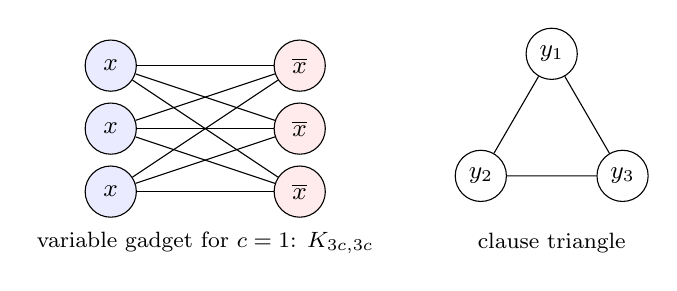
\begin{tikzpicture}[v/.style={circle,draw,minimum size=6.5mm,inner sep=0pt,font=\small}]
  \foreach \i in {1,2,3}{
    \node[v,fill=blue!8] (x\i) at (0,1.6-0.8*\i) {$x$};
    \node[v,fill=red!8] (n\i) at (2.4,1.6-0.8*\i) {$\overline{x}$};}
  \foreach \i in {1,2,3}{\foreach \j in {1,2,3}{\draw (x\i)--(n\j);}}
  \node[font=\footnotesize] at (1.2,-1.45) {variable gadget for $c=1$: $K_{3c,3c}$};
  \begin{scope}[shift={(5.6,0)}]
    \node[v] (a) at (0,0.95) {$y_1$};
    \node[v] (b) at (-0.9,-0.6) {$y_2$};
    \node[v] (c) at (0.9,-0.6) {$y_3$};
    \draw (a)--(b)--(c)--(a);
    \node[font=\footnotesize] at (0,-1.45) {clause triangle};
  \end{scope}
\end{tikzpicture}

{\footnotesize Every $x$-node is joined to every $\overline{x}$-node. A cut separating all $x$'s from all $\overline{x}$'s cuts all $(3c)^2$ edges; a triangle can contribute at most $2$ cut edges.}
\end{center}

\paragraph{Correctness.}
A consistent assignment of $x_i$ puts every $x_i$-node on one side of the cut and every $\overline{x}_i$-node on the other, contributing all $9c^2$ bipartite edges. Mixing the two parts of one variable yields a bipartite cut of size at most $9c^2-3c$ (the next-best splits differ by moving one node, which loses $3c$ edges). Each triangle contributes at most $2$ cut edges (a $2$--$1$ partition); all $c$ triangles contribute at most $2c$.

($\Rightarrow$) From a $\neq$-assignment, put every node labelled by a true literal in $S$ and every node labelled by a false literal in $T$. Each variable gadget is split cleanly: cut $9c^2 n$. Each clause has one or two true literals, so its triangle is split $2$--$1$: cut $2c$. Total $k$.

($\Leftarrow$) Suppose a cut of size $\ge k$ exists. Every variable gadget must be split cleanly: an inconsistent variable contributes $\le 9c^2-3c$, the others $\le 9c^2$, and triangles $\le 2c$, for a total $\le 9c^2 n-c<k$. The clean split defines an assignment ($x_i$ true iff the $x_i$-nodes lie in $S$). Variable gadgets then contribute exactly $9c^2 n$, so the triangles must contribute $\ge 2c$, hence exactly $2$ each. Each clause-triangle is $2$--$1$ across the cut, so the three literals are not all true and not all false: a $\neq$-assignment.

Theorem~7.36 gives $\NP$-completeness.
\end{soln}

\begin{question}{Problem 7.28}
You are given a box and a collection of cards as indicated in the following figure. Because of the pegs in the box and the notches in the cards, each card will fit in the box in either of two ways. Each card contains two columns of holes, some of which may not be punched out. The puzzle is solved by placing all the cards in the box so as to completely cover the bottom of the box (i.e., every hole position is blocked by at least one card that has no hole there). Let $\mathit{PUZZLE}=\{\enc{c_1,\dots,c_k}\mid \text{each $c_i$ represents a card and this collection of cards has a solution}\}$. Show that $\mathit{PUZZLE}$ is $\NP$-complete.
\begin{center}
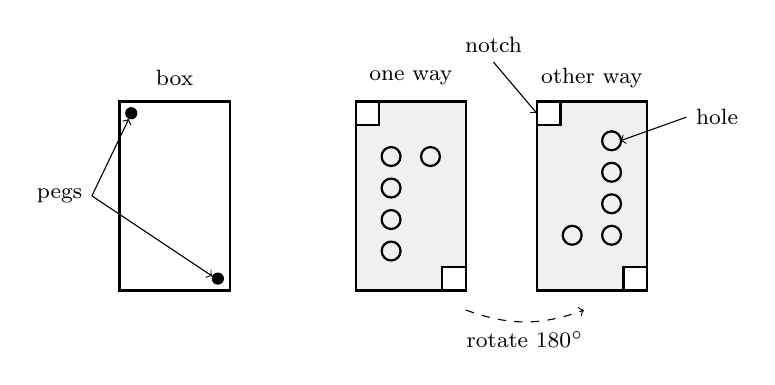
\begin{tikzpicture}[font=\footnotesize,hole/.style={draw,thick,circle,inner sep=0pt,minimum size=2.4mm}]
  \draw[thick] (0,0) rectangle (1.4,2.4);
  \fill (0.15,2.25) circle (2.2pt); \fill (1.25,0.15) circle (2.2pt);
  \node at (0.7,2.7) {box};
  \node[anchor=east] (pg) at (-0.35,1.2) {pegs};
  \draw[->] (pg.east) -- (0.12,2.18); \draw[->] (pg.east) -- (1.18,0.18);
  \foreach \dx/\lab/\L/\R in {3/one way/{0.5,0.9,1.3,1.7}/{1.7},5.3/other way/{0.7}/{0.7,1.1,1.5,1.9}}{
    \begin{scope}[shift={(\dx,0)}]
      \draw[thick,fill=black!6] (0,0) rectangle (1.4,2.4);
      \draw[thick,fill=white] (0,2.1) rectangle (0.3,2.4);
      \draw[thick,fill=white] (1.1,0) rectangle (1.4,0.3);
      \foreach \y in \L \node[hole] at (0.45,\y) {};
      \foreach \y in \R \node[hole] at (0.95,\y) {};
      \node at (0.7,2.7) {\lab};
    \end{scope}}
  \draw[<-] (5.3,2.25) -- (4.75,2.9) node[above] {notch};
  \draw[<-] (6.36,1.9) -- (7.2,2.2) node[right] {hole};
  \draw[->,dashed] (4.4,-0.25) to[bend right=20] node[below] {rotate $180^\circ$} (5.9,-0.25);
\end{tikzpicture}
\end{center}
\end{question}
\begin{soln}
\textbf{Idea.} Each card is a variable and its two placements are truth values. A $180^\circ$ rotation (the two ways the notches meet the pegs) swaps the two columns and reverses the rows; making each column a palindrome cancels the reversal, so a placement is just a column-swap. Positions in the left column encode ``some literal is true'' and those in the right encode ``some literal is false'', i.e.\ a $\neq$-assignment.



\paragraph{In $\NP$.}
Certificate: a bit for each card (which of the two placements). Verifier lays the cards (applying a $180^\circ$ rotation where the bit says so) and checks that every grid position is solid on at least one card. Time polynomial in the total number of hole-positions.

\paragraph{Hardness.}
Reduce $\neq\mathrm{SAT}$ (Problem~7.26) to $\mathit{PUZZLE}$. Let $\phi$ have variables $x_1,\dots,x_n$ and clauses $c_1,\dots,c_m$. One card per variable. The grid has two columns and $2m$ rows: rows $1,\dots,m$ index the clauses, and row $2m+1-j$ is a copy of row $j$, so each column is a palindrome. Then a $180^\circ$ rotation equals a swap of the two columns.

For the card of $x_i$, in the ``true'' orientation:
\begin{enumerate}
\item Left column, row $j$ (and its palindromic copy): \emph{solid} iff $x_i$ occurs positively in clause $c_j$; punched otherwise.
\item Right column, row $j$ (and copy): \emph{solid} iff $\overline{x}_i$ occurs in $c_j$; punched otherwise.
\end{enumerate}
The ``false'' placement is the $180^\circ$ rotation, which puts the old right column on the left.

($\Rightarrow$) From a $\neq$-assignment, place card $x_i$ in the true orientation iff $x_i$ is true. Left column, row $j$ is solid on some card iff some true literal occurs in $c_j$. Right column, row $j$ is solid iff some false literal occurs in $c_j$. A $\neq$-assignment gives both, so every position is blocked. Palindromic copies are blocked for the same reason.

($\Leftarrow$) From a solution, set $x_i$ true iff card $x_i$ is in the true orientation. For each clause $c_j$, the left (resp.\ right) position in row $j$ is blocked, so some true (resp.\ false) literal occurs in $c_j$: a $\neq$-assignment.

The cards are of size $O(m)$ and there are $n$ of them, so the reduction is polynomial. Theorem~7.36 gives $\NP$-completeness.
\end{soln}

\begin{question}{Problem 7.29}
A \emph{coloring} of a graph is an assignment of colors to its nodes so that no two adjacent nodes are assigned the same color. Let
\[
3\mathrm{COLOR}=\{\enc{G}\mid G\text{ is colorable with $3$ colors}\}.
\]
Show that $3\mathrm{COLOR}$ is $\NP$-complete. (Hint: Use the following three subgraphs.)
\begin{center}
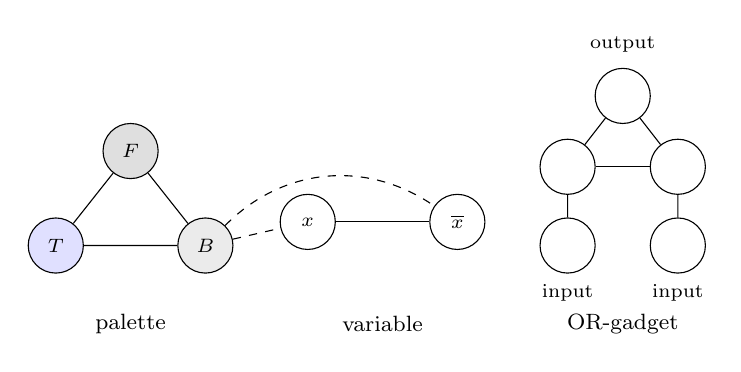
\begin{tikzpicture}[
  v/.style={circle, draw, minimum size=7mm, inner sep=0pt, font=\scriptsize}]
  \node[v, fill=blue!12] (T) at (0,0) {$T$};
  \node[v, fill=gray!25] (Fcol) at (0.95,1.2) {$F$};
  \node[v, fill=black!8] (B) at (1.9,0) {$B$};
  \draw (T)--(Fcol)--(B)--(T);
  \node[font=\footnotesize] at (0.95,-1.0) {palette};
  \node[v] (x) at (3.2,0.3) {$x$};
  \node[v] (nx) at (5.1,0.3) {$\overline{x}$};
  \draw (x)--(nx);
  \draw[dashed] (B)--(x);
  \draw[dashed] (B) to[bend left=40] (nx);
  \node[font=\footnotesize] at (4.15,-1.0) {variable};
  \begin{scope}[shift={(6.5,0)}]
    \node[v] (in1) at (0,0) {};
    \node[v] (in2) at (1.4,0) {};
    \node[v] (p) at (0,1.0) {};
    \node[v] (q) at (1.4,1.0) {};
    \node[v] (w) at (0.7,1.9) {};
    \draw (in1)--(p)--(w)--(q)--(in2);
    \draw (p)--(q);
    \node[font=\footnotesize] at (0.7,-1.0) {OR-gadget};
    \node[font=\scriptsize] at (0,-0.6) {input};
    \node[font=\scriptsize] at (1.4,-0.6) {input};
    \node[font=\scriptsize] at (0.7,2.55) {output};
  \end{scope}
\end{tikzpicture}
\end{center}
\end{question}
\begin{soln}
\textbf{Idea.} A palette triangle names the three colors $T,F,B$. Each variable is a pair of nodes adjacent to each other and to $B$, so they receive $\{T,F\}$. An OR-gadget (the book's third subgraph) outputs $T$ iff at least one input is $T$; cascading two of them per clause and pinning the output to $T$ enforces the clause.

\paragraph{In $\NP$.}
Certificate: a map $c\colon V\to\{1,2,3\}$. Verifier checks $c(u)\neq c(v)$ on every edge. Time $O(|E|)$.

\paragraph{Hardness.}
Reduce $3\mathrm{SAT}$ (Corollary~7.42) to $3\mathrm{COLOR}$. Let $\phi$ have variables $x_1,\dots,x_n$ and clauses $c_1,\dots,c_m$. Build $G$ from the three book gadgets.



\begin{enumerate}
\item \emph{Palette.} A triangle on nodes $T,F,B$. In any $3$-coloring these three nodes receive three different colors; name the colors after the nodes.
\item \emph{Variable gadgets.} For each $x_i$, two nodes $x_i$ and $\overline{x}_i$, with edges $\{x_i,\overline{x}_i\}$, $\{x_i,B\}$, $\{\overline{x}_i,B\}$. Both are adjacent to $B$, so they are colored $T$ or $F$; they are adjacent to each other, so they receive opposite colors. That is the assignment.
\item \emph{OR-gadget.} Five nodes: inputs $a,b$, internals $p,q$, output $w$, and edges $\{a,p\}$, $\{b,q\}$, $\{p,q\}$, $\{p,w\}$, $\{q,w\}$. Identify $a,b$ with existing literal nodes (already colored $T$ or $F$).
\end{enumerate}

\paragraph{OR-gadget property.}
Assume $a,b\in\{T,F\}$.
\begin{itemize}
\item If $a=b=F$, then $p,q\in\{T,B\}$ and $p\neq q$, so $\{p,q\}=\{T,B\}$ and $w$ (adjacent to both) is $F$.
\item If $a=b=T$, symmetrically $w$ is forced $T$.
\item If $a=T$ and $b=F$, the coloring $p=F$, $q=B$, $w=T$ is legal, so $w$ \emph{can} be $T$. (Other colors for $w$ are also possible.)
\end{itemize}
Thus: $w$ is forced $F$ if both inputs are $F$; and if at least one input is $T$, there is a coloring of the gadget with $w=T$. Connecting $w$ to $B$ keeps $w\in\{T,F\}$ without destroying the ``$w$ can be $T$'' coloring ($q=B$ is an internal node, not adjacent to the palette $B$).

\paragraph{Clauses.}
For $c_j=(y_1\lor y_2\lor y_3)$, attach an OR-gadget with inputs $y_1,y_2$ and output $o_j$, connect $o_j$ to $B$, then a second OR-gadget with inputs $o_j,y_3$ and output $w_j$. Connect $w_j$ to both $F$ and $B$, forcing $w_j=T$. By the property, $w_j=T$ is possible iff $y_1\lor y_2\lor y_3$ is true under the variable coloring.

($\Rightarrow$) From a satisfying assignment, color $x_i$ with $T$ or $F$ accordingly, color the palette, and color each OR-gadget as in the property so every clause output is $T$.

($\Leftarrow$) From a $3$-coloring, the palette names the colors, each variable gadget is an assignment, and each clause output $w_j=T$ implies that clause is satisfied.

The graph has $O(n+m)$ nodes and edges. Theorem~7.36 gives $\NP$-completeness.
\end{soln}

\begin{question}{Problem 7.30}
Let $\mathit{SET\text{-}SPLITTING}$ be the language of encodings $\enc{S,C}$ where $S$ is a finite set and $C=\{C_1,\dots,C_k\}$ is a collection of subsets of $S$, for some $k>0$, such that the elements of $S$ can be colored red or blue so that no $C_i$ is monochromatic. Show that $\mathit{SET\text{-}SPLITTING}$ is $\NP$-complete.
\end{question}
\begin{soln}
\textbf{Idea.} This is hypergraph $2$-coloring. A $\neq$-assignment is a $2$-coloring of literals that splits every clause; copy each variable into a true-token and a false-token that must receive opposite colors.

\paragraph{In $\NP$.}
Certificate: a coloring $S\to\{\mathrm{red},\mathrm{blue}\}$. Verifier checks each $C_i$ contains both colors. Time $O(\sum_i|C_i|)$.

\paragraph{Hardness.}
Reduce $\neq\mathrm{SAT}$ (Problem~7.26) to $\mathit{SET\text{-}SPLITTING}$. Let $\phi$ have variables $x_1,\dots,x_n$ and clauses $c_1,\dots,c_m$. Set
\[
S=\{x_1^T,x_1^F,\dots,x_n^T,x_n^F\}
\]
and let $C$ contain
\begin{enumerate}
\item the pair $\{x_i^T,x_i^F\}$ for each $i$ (so the two tokens get opposite colors);
\item for each clause, the $3$-set of tokens of its literals, where the token of $x_i$ is $x_i^T$ and the token of $\overline{x}_i$ is $x_i^F$.
\end{enumerate}

($\Rightarrow$) From a $\neq$-assignment, color a token red iff the corresponding literal is true. Each pair $\{x_i^T,x_i^F\}$ is split. Each clause has a true and a false literal, so its $3$-set is split.

($\Leftarrow$) From a red/blue coloring that splits every set of $C$, each pair $\{x_i^T,x_i^F\}$ is bichromatic. Set $x_i$ true iff $x_i^T$ is red. Then a literal-token is red iff that literal is true, so each clause $3$-set being split means the three literals are not all equal: a $\neq$-assignment.

The instance has size $O(n+m)$. Theorem~7.36 gives $\NP$-completeness.
\end{soln}

\begin{question}{Problem 7.31}
Consider the following scheduling problem. You are given a list of final exams $F_1,\dots,F_k$ to be scheduled, and a list of students $S_1,\dots,S_\ell$. Each student is taking some specified subset of these exams. You must schedule these exams into slots so that no student is required to take two exams in the same slot. The problem is to determine if such a schedule exists that uses only $h$ slots. Formulate this problem as a language and show that this language is $\NP$-complete.
\end{question}
\begin{soln}
\textbf{Idea.} The conflict graph (exams as vertices, an edge when some student takes both) must be $h$-colorable. Hardness is $3\mathrm{COLOR}$ (Problem~7.29) with $h=3$, one student per edge.

Let $\mathit{EXAM}$ be the language of encodings $\enc{F_1,\dots,F_k,\; S_1,\dots,S_\ell,\; h}$ where each student $S_j$ is a specified subset of the exams, and the exams can be assigned to at most $h$ slots so that no student takes two exams in the same slot.

\paragraph{In $\NP$.}
Certificate: a function $\sigma\colon\{F_1,\dots,F_k\}\to\{1,\dots,h\}$. Verifier checks the range, and that no student set contains two exams with equal $\sigma$. Time polynomial in the input length.

\paragraph{Hardness.}
Reduce $3\mathrm{COLOR}$ (Problem~7.29) to $\mathit{EXAM}$. Given $G=(V,E)$, create one exam $F_v$ per vertex, one student $S_e$ per edge $e=\{u,v\}$ who takes exactly $\{F_u,F_v\}$, and set $h=3$. A $3$-coloring of $G$ is a $3$-slot schedule with no student conflict, and conversely. The map is linear in $|V|+|E|$. Theorem~7.36 gives $\NP$-completeness.

(Equivalently: $\mathit{EXAM}$ is the language of $h$-colorable conflict graphs, and $3$-colorability is $\NP$-complete.)
\end{soln}

\begin{question}{Problem 7.32}
This problem is inspired by the single-player game Minesweeper, generalized to an arbitrary graph. Let $G$ be an undirected graph, where each node either contains a single, hidden mine or is empty. The player chooses nodes, one by one. If the player chooses a node containing a mine, the player loses. If the player chooses an empty node, the player learns the number of neighboring nodes containing mines. (A neighboring node is one connected to the chosen node by an edge.) The player wins if and when all empty nodes have been so chosen.

In the \emph{mine consistency problem}, you are given a graph $G$ along with numbers labeling some of $G$'s nodes. You must determine whether a placement of mines on the remaining nodes is possible, so that any node $v$ that is labeled $m$ has exactly $m$ neighboring nodes containing mines. Formulate this problem as a language and show that it is $\NP$-complete.
\end{question}
\begin{soln}
\textbf{Idea.} Labeled nodes are revealed empties: they have no mine, and their number is the count of mined neighbors. A variable is two unlabeled nodes with a common neighbor labelled $1$ (exactly one mine). A clause is a node labelled $3$ adjacent to the three literals and two slack nodes, so $1$, $2$, or $3$ of the literals may be mined.

Let $\mathit{MINECONS}$ be the language of encodings $\enc{G,\lambda}$ where $\lambda$ labels some nodes of $G$ with natural numbers, and there is a set $M$ of \emph{unlabelled} nodes (the mines) such that every labelled $v$ has exactly $\lambda(v)$ neighbors in $M$. Labelled nodes are not mined.

\paragraph{In $\NP$.}
Certificate: the set $M$ of mined (unlabelled) nodes. Verifier checks that no labelled node is in $M$, and that each labelled $v$ has exactly $\lambda(v)$ neighbors in $M$. Time $O(|E|)$.

\paragraph{Hardness.}
Reduce $3\mathrm{SAT}$ to $\mathit{MINECONS}$. Let $\phi$ have variables $x_1,\dots,x_n$ and clauses $c_1,\dots,c_m$.

\begin{center}
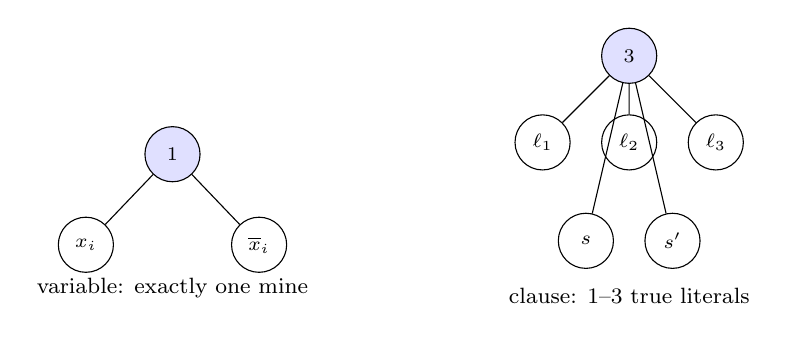
\begin{tikzpicture}[
  u/.style={circle, draw, minimum size=7mm, inner sep=0pt, font=\scriptsize},
  labn/.style={circle, draw, fill=blue!12, minimum size=7mm, inner sep=0pt, font=\scriptsize}]
  \node[u] (x) at (0,0) {$x_i$};
  \node[u] (nx) at (2.2,0) {$\overline{x}_i$};
  \node[labn] (ui) at (1.1,1.15) {$1$};
  \draw (x)--(ui)--(nx);
  \node[font=\footnotesize] at (1.1,-0.55) {variable: exactly one mine};
  \begin{scope}[shift={(5.8,0.2)}]
    \node[u] (l1) at (0,1.1) {$\ell_1$};
    \node[u] (l2) at (1.1,1.1) {$\ell_2$};
    \node[u] (l3) at (2.2,1.1) {$\ell_3$};
    \node[u] (s1) at (0.55,-0.15) {$s$};
    \node[u] (s2) at (1.65,-0.15) {$s'$};
    \node[labn] (C) at (1.1,2.2) {$3$};
    \draw (C)--(l1) (C)--(l2) (C)--(l3) (C)--(s1) (C)--(s2);
    \node[font=\footnotesize] at (1.1,-0.85) {clause: $1$--$3$ true literals};
  \end{scope}
\end{tikzpicture}
\end{center}

\begin{enumerate}
\item For each $x_i$: unlabeled nodes $x_i,\overline{x}_i$ and a node $u_i$ labelled $1$, adjacent only to $x_i$ and $\overline{x}_i$. Then $M$ contains exactly one of $x_i,\overline{x}_i$.
\item For each clause $c_j=(\ell_1\lor\ell_2\lor\ell_3)$: a node $C_j$ labelled $3$, adjacent to the three literal-nodes (identifying $\ell$ with $x_i$ or $\overline{x}_i$) and to two fresh unlabeled slack nodes $s_j,s'_j$. Then $|M\cap\{\ell_1,\ell_2,\ell_3,s_j,s'_j\}|=3$. With only two slacks, this is possible iff at least one literal-node is mined, and it is possible for $1$, $2$, or $3$ mined literals (fill with slacks).
\end{enumerate}

($\Rightarrow$) From a satisfying assignment, mine the true literal-node of each variable, and for each clause mine enough slacks to bring the neighbor-count of $C_j$ to $3$.

($\Leftarrow$) From a consistent mine placement, exactly one of $x_i,\overline{x}_i$ is mined: that is an assignment. Each $C_j$ has three mined neighbors among five, so at least one literal is mined: the assignment satisfies $\phi$.

The graph has $O(n+m)$ nodes. Theorem~7.36 gives $\NP$-completeness.
\end{soln}

\begin{question}{Problem 7.33}
In the following solitaire game, you are given an $m\times m$ board. On each of its $m^2$ positions lies either a blue stone, a red stone, or nothing at all. You play by removing stones from the board until each column contains only stones of a single color and each row contains at least one stone. You win if you achieve this objective. Winning may or may not be possible, depending upon the initial configuration. Let $\mathit{SOLITAIRE}=\{\enc{G}\mid G\text{ is a winnable game configuration}\}$. Prove that $\mathit{SOLITAIRE}$ is $\NP$-complete.
\end{question}
\begin{soln}
\textbf{Idea.} Columns are variables (keep blue $=$ true, keep red $=$ false). Rows are clauses: a remaining stone in row $c_j$ is a true literal of that clause. (This is the book's selected solution.)

\paragraph{In $\NP$.}
Certificate: the set of stones that remain. Verifier checks they were present initially, each nonempty column is monochromatic, and every row still has a stone. Time $O(m^2)$.

\paragraph{Hardness.}
Reduce $3\mathrm{SAT}$ to $\mathit{SOLITAIRE}$. Let $\phi$ have variables $x_1,\dots,x_m$ and clauses $c_1,\dots,c_k$. Delete any clause containing both $x_i$ and $\overline{x}_i$ (such a clause is a tautology). Build a $k\times m$ board: row $c_j$, column $x_i$ gets a blue stone if $x_i$ occurs in $c_j$, a red stone if $\overline{x}_i$ occurs in $c_j$, and nothing otherwise. Pad to a square by repeating a row or adding a blank column; neither changes winnability (a repeated row is satisfied iff the original is; a blank column can be emptied). Output this board $G$.

\begin{center}
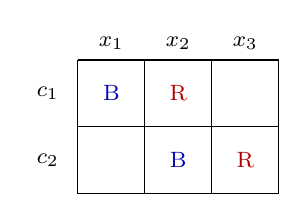
\begin{tikzpicture}[font=\footnotesize, scale=0.85]
  \draw (0,0) grid (3,2);
  \node at (0.5,1.5) {\textcolor{blue!70!black}{B}};
  \node at (1.5,1.5) {\textcolor{red!70!black}{R}};
  \node at (2.5,1.5) {};
  \node at (0.5,0.5) {};
  \node at (1.5,0.5) {\textcolor{blue!70!black}{B}};
  \node at (2.5,0.5) {\textcolor{red!70!black}{R}};
  \node at (-0.45,1.5) {$c_1$};
  \node at (-0.45,0.5) {$c_2$};
  \node at (0.5,2.25) {$x_1$};
  \node at (1.5,2.25) {$x_2$};
  \node at (2.5,2.25) {$x_3$};
\end{tikzpicture}
\end{center}
A tiny example: $(x_1\lor\overline{x}_2)\land(x_2\lor\overline{x}_3)$. Keeping blue in column $x_1$, red in $x_2$, blue in $x_3$ leaves a stone in every row.

($\Rightarrow$) From a satisfying assignment: if $x_i$ is true (false), remove all red (blue) stones from column $x_i$. Remaining stones are true literals. Each clause has a true literal, so each row has a stone, and each column is monochromatic.

($\Leftarrow$) From a winning configuration: if red (blue) stones were removed from a column, set that variable true (false); if the column is empty, assign arbitrarily. Every row still has a stone, so every clause has a true literal.

The board has size $O((k+m)^2)$, polynomial. Theorem~7.36 gives $\NP$-completeness.
\end{soln}

\begin{question}{Problem 7.34}
Recall, in our discussion of the Church--Turing thesis, that we introduced the language $D=\{\enc{p}\mid p\text{ is a polynomial in several variables having an integral root}\}$. We stated, but didn't prove, that $D$ is undecidable. In this problem, you are to prove a different property of $D$---namely, that $D$ is $\NP$-hard. A problem is $\NP$-hard if all problems in $\NP$ are polynomial time reducible to it, even though it may not be in $\NP$ itself. So you must show that all problems in $\NP$ are polynomial time reducible to $D$.
\end{question}
\begin{soln}
\textbf{Idea.} $3\mathrm{SAT}$ is $\NP$-complete, so it is enough to write a polynomial that vanishes over the integers iff a given $3$cnf-formula is satisfiable: force $0$-$1$ values with $x(x-1)=0$, and force each clause with a product that is zero iff some literal is true.

By Corollary~7.42 and Theorem~7.36 (composability of $\le_{\mathrm{P}}$, Theorem~7.31's companions in Definitions~7.29 and~7.34), every language in $\NP$ polynomial-time reduces to $3\mathrm{SAT}$. We give $3\mathrm{SAT}\redp D$.

Given a $3$cnf-formula $\phi$ with variables $x_1,\dots,x_n$ and clauses $c_1,\dots,c_m$, produce the polynomial
\[
p(x_1,\dots,x_n)
=\sum_{i=1}^n \bigl(x_i(x_i-1)\bigr)^2
+\sum_{j=1}^m \bigl((1-y_{j1})(1-y_{j2})(1-y_{j3})\bigr)^2,
\]
where $y_{jr}$ is $x_i$ if the $r$-th literal of $c_j$ is $x_i$, and $1-x_i$ if it is $\overline{x}_i$. Output $\enc{p}$. Expanding each small square gives $O(1)$ monomials per summand, so $|\enc{p}|$ is $O(|\enc{\phi}|)$ and the map is polynomial time.

\paragraph{Correctness.}
If $a\in\mathbb{Z}^n$ is a root, each square vanishes, so each $a_i\in\{0,1\}$ and each clause has some $y_{jr}=1$, i.e.\ $\phi$ is satisfied.

Conversely, a satisfying $0$-$1$ assignment is an integral root.

Thus $\phi$ is satisfiable iff $\enc{p}\in D$. Every language in $\NP$ therefore reduces to $D$, so $D$ is $\NP$-hard.

(Note: $D$ is undecidable, hence not in $\NP$, so it is not $\NP$-complete.)
\end{soln}

\begin{question}{Problem 7.35}
A subset of the nodes of a graph $G$ is a \emph{dominating set} if every other node of $G$ is adjacent to some node in the subset. Let
\[
\mathit{DOMINATING\text{-}SET}=\{\enc{G,k}\mid G\text{ has a dominating set with $k$ nodes}\}.
\]
Show that it is $\NP$-complete by giving a reduction from $\mathit{VERTEX\text{-}COVER}$.
\end{question}
\begin{soln}
\textbf{Idea.} Turn every edge into a triangle by adding a pendant midpoint. A vertex cover of $G$ dominates all midpoints; conversely, midpoints in a dominating set can be swapped for an endpoint, yielding a vertex cover of the same size. Isolated vertices are deleted first (they do not affect vertex cover, but must belong to every dominating set).

\paragraph{In $\NP$.}
Certificate: a set $D$ of $k$ nodes. Verifier checks that every node outside $D$ has a neighbor in $D$. Time $O(|E|)$.

\paragraph{Hardness.}
Reduce $\mathit{VERTEX\text{-}COVER}$ (Theorem~7.44) to $\mathit{DOMINATING\text{-}SET}$. Given $\enc{G,k}$:
\begin{enumerate}
\item If $k>|V(G)|$, output a fixed no-instance (neither language then contains the input).
\item Delete all isolated vertices of $G$ (a vertex cover never needs them, so membership is unchanged). If nothing remains, output a yes-instance iff $k\ge 0$.
\item Form $G'$ by keeping every vertex and edge of $G$ and, for each edge $e=\{u,v\}$, adding a new vertex $x_e$ adjacent to both $u$ and $v$ (so $\{u,v,x_e\}$ is a triangle).
\item Output $\enc{G',k}$.
\end{enumerate}

\begin{center}
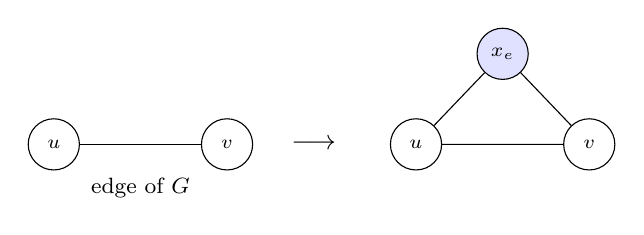
\begin{tikzpicture}[
  v/.style={circle, draw, minimum size=6.5mm, inner sep=0pt, font=\scriptsize}]
  \node[v] (u) at (0,0) {$u$};
  \node[v] (w) at (2.2,0) {$v$};
  \draw (u)--(w);
  \node[font=\footnotesize] at (1.1,-0.55) {edge of $G$};
  \node at (3.3,0) {$\longrightarrow$};
  \begin{scope}[shift={(4.6,0)}]
    \node[v] (u2) at (0,0) {$u$};
    \node[v] (w2) at (2.2,0) {$v$};
    \node[v, fill=blue!12] (xe) at (1.1,1.15) {$x_e$};
    \draw (u2)--(w2)--(xe)--(u2);
  \end{scope}
\end{tikzpicture}
\end{center}

($\Rightarrow$) Let $C$ be a $k$-node vertex cover of $G$. Then $C$ dominates $G'$: each $x_e$ is adjacent to an endpoint in $C$; each original $v\notin C$ has an incident edge (no isolates) whose other end lies in $C$, and that edge remains in $G'$.

($\Leftarrow$) Let $D$ be a $k$-node dominating set of $G'$. For every $x_e\in D$, replace $x_e$ by an endpoint of $e$ not already in $D$ (if both endpoints are already in, just drop $x_e$). The resulting $C\subseteq V(G)$ has $|C|\le k$. For each edge $e=\{u,v\}$, the vertex $x_e$ is dominated by $D$, so $D$ meets $\{u,v,x_e\}$; after the swap, $C$ meets $\{u,v\}$. Thus $C$ is a vertex cover. A superset of a vertex cover is a vertex cover, and $k\le|V(G)|$, so we may add vertices to $C$ to obtain a $k$-node vertex cover of $G$.

The construction is polynomial. Theorem~7.36 gives $\NP$-completeness.
\end{soln}

\begin{question}{Problem 7.36 $\bigstar$}
Show that the following problem is $\NP$-complete. You are given a set of states $Q=\{q_0,q_1,\dots,q_\ell\}$ and a collection of pairs $\{(s_1,r_1),\dots,(s_k,r_k)\}$ where the $s_i$ are distinct strings over $\Sigma=\{0,1\}$, and the $r_i$ are (not necessarily distinct) members of $Q$. Determine whether a DFA $M=(Q,\Sigma,\delta,q_0,F)$ exists where $\delta(q_0,s_i)=r_i$ for each $i$. Here, $\delta(q,s)$ is the state that $M$ enters after reading $s$, starting at state $q$. (Note that $F$ is irrelevant here.)
\end{question}
\begin{soln}
\textbf{Idea.} The transition table $\delta$ is a polynomial certificate. For hardness, encode a $3$-coloring: string $1^i$ reaches a vertex-state $s_i$, and the unknown bit $\delta(s_i,0)$ is the color of $v_i$, forced into a $3$-state core. Adjacent vertices are given incompatible $1$-continuations from their color-chains, so they cannot share a color.

Call the language $\mathit{DFA\text{-}TRACE}$: encodings of a state set $Q$ and pairs $\{(s_i,r_i)\}$ for which some $\delta\colon Q\times\{0,1\}\to Q$ satisfies $\widehat{\delta}(q_0,s_i)=r_i$ for every $i$.

\paragraph{In $\NP$.}
Certificate: the table $\delta$ (size $2|Q|$). Verifier, for each pair, walks $s_i$ from $q_0$ and checks the state is $r_i$. Time $O\bigl(|Q|+\sum_i|s_i|\bigr)$.

\paragraph{Hardness.}
Reduce $3\mathrm{COLOR}$ (Problem~7.29) to $\mathit{DFA\text{-}TRACE}$. Let $G=(V,E)$ with $V=\{v_1,\dots,v_n\}$ and $E=\{e_1,\dots,e_m\}$. If $m=0$, output the trivial yes-instance $Q=\{q_0\}$ with no pairs (every graph with no edges is $3$-colorable). Assume $m\ge 1$.

\emph{States.} $Q$ contains $q_0$, merge/sink states $M,F$, vertex states $s_1,\dots,s_n$, color states $c_1,c_2,c_3$, chain states $p_{a,j}$ for $a\in\{1,2,3\}$ and $1\le j\le m$, and terminals $t_+,t_-$.

\emph{Pairs, in groups.}
\begin{enumerate}
\item \emph{Vertex chain.} For $i=1,\dots,n$: $1^i\mapsto s_i$. Thus $\delta(q_0,1)=s_1$ and $\delta(s_i,1)=s_{i+1}$ (with $s_{n}$ looping or going to $q_0$ on a further $1$, unused).
\item \emph{Color core, reached on $0$-prefixes.}
$0\mapsto c_1$,\quad
$01\mapsto c_2$,\quad
$011\mapsto c_3$.
So $\delta(q_0,0)=c_1$, $\delta(c_1,1)=c_2$, $\delta(c_2,1)=c_3$.
\item \emph{Private $0$-chains} of length $m$ from each color, then merge at $M$:
for $a=1,2,3$ and $j=1,\dots,m$, the string that reaches $c_a$ followed by $0^j$ maps to $p_{a,j}$; one more $0$ maps to $M$; then $0$ maps to $F$ and stays ($F$ is a $0$-sink). Concretely:
$0^{j+1}\mapsto p_{1,j}$,\quad
$0^{m+2}\mapsto M$,\quad
$0^{m+3}\mapsto F$,\quad
$0^{m+4}\mapsto F$,
and the analogous strings $01\,0^j\mapsto p_{2,j}$, $011\,0^j\mapsto p_{3,j}$.
\item \emph{Membership.} $1^i\,0^{m+2}\mapsto M$ for each $i$. This forces $\delta(s_i,0)$ to be a state that reaches $M$ after exactly $m+1$ zeros (see below).
\item \emph{Edge tests.} For each edge $e_j=\{v_r,v_s\}$ with $r<s$:
\[
1^r\,0^{j+1}\,1\;\mapsto\; t_+,\qquad
1^s\,0^{j+1}\,1\;\mapsto\; t_-.
\]
Path: $1^r$ to $s_r$, then $0$ to the color $c_a$, then $0^j$ to $p_{a,j}$, then $1$ to the terminal.
\item \emph{Pin the terminals.} For the first edge $e_1=\{v_r,v_s\}$ add $1^r\,0^{2}\,1\,0\mapsto F$ and $1^s\,0^{2}\,1\,0\mapsto F$. This forces $\delta(t_+,0)=\delta(t_-,0)=F$.
\end{enumerate}

\textbf{Why item~(4) forces a genuine color.} After item~(6), the only states whose $0$-transition is not fixed are the vertex states $s_k$. Following $0$'s: $c_a$ reaches $M$ after exactly $m+1$ steps; $p_{a,j}$ after $m+1-j$; $q_0$ after $m+2$; from $M,F,t_\pm$ the walk falls into the $0$-sink $F$ and never returns to $M$; and each $s_k$ needs $m+2$ (by its own item-(4) pair). So $\delta(s_i,0)$ must be one of $c_1,c_2,c_3$. (Without item~(6) a vertex could ``hide'' at $t_\pm$ and use it as a fourth color.)

\paragraph{Correctness.}
($\Rightarrow$) Given a $3$-coloring $\chi\colon V\to\{1,2,3\}$, set $\delta(s_i,0)=c_{\chi(v_i)}$. For each edge $e_j=\{v_r,v_s\}$ set $\delta(p_{\chi(v_r),j},1)=t_+$ and $\delta(p_{\chi(v_s),j},1)=t_-$; unused $(a,j)$ send $1$ to $M$. All other transitions are the ones forced by the pairs above (or to $M$). Adjacent vertices have different colors, so the two $1$-transitions from the corresponding $p_{a,j}$ do not clash. Every listed pair holds.

($\Leftarrow$) Given any $\delta$ meeting the pairs, item~(4) forces $\chi(v_i):=\delta(s_i,0)\in\{c_1,c_2,c_3\}$. If some edge $e_j=\{v_r,v_s\}$ had $\chi(v_r)=\chi(v_s)=c_a$, then both $1^r 0^{j+1}1$ and $1^s 0^{j+1}1$ would walk to the same state $p_{a,j}$ and then on $1$ to the same place, contradicting $t_+\neq t_-$. So $\chi$ is a $3$-coloring.

The instance has $|Q|=O(n+m)$ and $O(n+m)$ pairs of polynomial length. Theorem~7.36 gives $\NP$-completeness.
\end{soln}
